\section{Bonusprogramme}
Bonusprogramme unterscheiden sich in Cashback und Payback (Treuepunkte). \newline

\noindent Bei Payback werden Treuepunkte gesammelt, die anschließend ab einer gewissen Punkteanzahl in Gutscheine bzw. Voucher eingelöst werden können. Zum Beispiel bei Fluglinien können Personen Flugmeilen sammeln, welche für Freiflüge, Upgrades, Hotelübernachtungen oder Mietwagen eingelöst werden können. Bei Payback bleibt das Geld bzw. die Leistung im Kreislauf des beteiligten Unternehmens. \cite{paycashback_all} \newline

\noindent \textit{``Ob beim Shoppen, Fliegen, Tanken oder Telefonieren: Mit dem Prinzip des Punktesammelns über Payback, Webmiles oder Kundenkarten wie die DeutschlandCard sind Verbraucher in der Offline-Welt seit Jahren bestens vertraut. Mit dem Aufkommen des E-Commerce haben findige Anbieter das Modell der Bonusprogramme erfolgreich in die Onlinewelt übertragen – die Idee des Cashbacks war geboren. Vorreitermärkte sind weltweit die USA und Großbritannien. In Kontinentaleuropa hinkt Cashback hingegen noch hinterher – das Potenzial wird insbesondere im deutschen Markt noch unterschätzt. Doch durch die Verbreitung mobiler Endgeräte steigert sich das Potenzial zusätzlich.'' \cite{Bonus_affiliate}} \newline

\noindent Beim Cashback bekommt der Kunde bares Geld zurück, welches er woanders wieder investieren kann. Einige Cashback Anbieter erhalten eine Provision durch sogenannte Affiliate Links, in dem über das Portal der Verkauf bestätigt wird. \cite{cashback-vergleich} \newline

\noindent Für den Erhalt des Geldes muss der Kunde/ Teilnehmer seine Kontodaten bekanntgeben. \cite{paycashback_all} \newline

\begin{figure}[!ht]
	\centering
	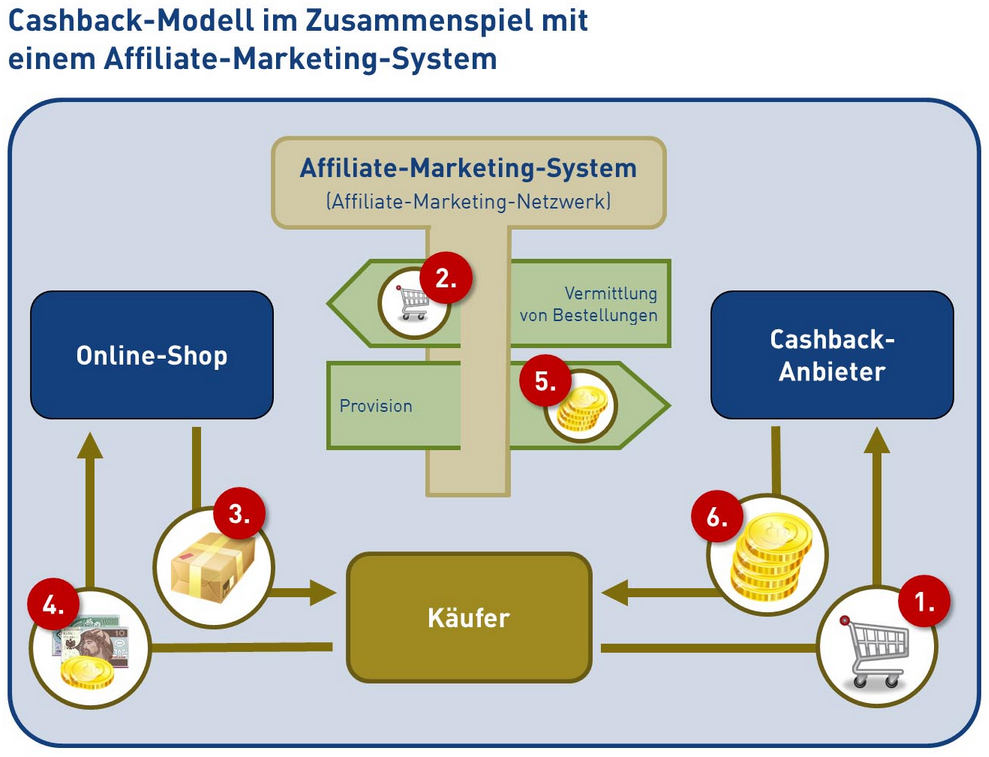
\includegraphics[width=0.8\textwidth]{Cashback-Modell im Zusammenhang mit einem Affiliate-Marketing-System}
	\caption{Cashback-Modell im Zusammenhang mit einem Affiliate-Marketing-System \cite{Bonus_affiliate} }
	\label{fig:Bonus_affiliate}
\end{figure}
\FloatBarrier

\begin{enumerate}
	\item Kunde kauft über ein Cashback-Anbieter in einem Online-Shop ein.
	\item Die Bestellung wird über das Affiliate-Netzwerk an den Online-Shop übermittelt.
	\item Der Online-Shop versendet die Ware an den Käufer.
	\item Der Käufer zahlt an den Online-Shop.
	\item Der Online-Shop zahlt die Provision über das Affiliate-Netzwerk an den Cashback-Anbieter.
	\item Der Cashback-Anbieter zahlt an den Käufer den Einkaufsrabatt (Cashback) \cite{Bonus_affiliate}
\end{enumerate}

\noindent Der wesentliche Unterschied zwischen Cashback und Payback liegt darin, das mit Cashback direkt nach jedem Einlauf Geld erstattet wird, welcher auf das Bankkonto des Kunden gutgeschrieben wird. Zum Beispiel gibt es Aktionen 3 für 2 (1x wird direkt ausgezahlt) im Einzelhandel von Weichspüler oder Schokolade. Dazu muss man in dem Aktionszeitraum die Produkte einkaufen und anschließend den Kassenzettel hochladen. Danach bekommt man das Geld erstattet, welches zuerst vom Kunden ausgegeben wurde. Payback kann erst im Anschluss ab einer gewissen Punktemenge in Prämien oder Gutscheinen eingelöst werden. \cite{TreueCash} \newline

\noindent Es gibt verschiedene Anbieter für Bonusprogramme z.B. für Treuepunkte sei genannt DeutschlandCard, Payback, Webmiles, KauflandCard, DM. Für Cashback-Programme z. B. card4you, Shoop. Weiterhin existieren noch viele weitere Anbieter, in dieser Arbeit wird im Punkt \ref{Payback} auf Payback eingegangen und die KauflandCard.

\subsection {Ziele}
Die Ziele von Bonusprogrammen sind: \newline

\noindent \textbf{Kundenbindung:} \textit{``Bei Payback und Cashback erhalten Kunden für ihren Einkauf Prämien, Gutscheine oder bares Geld zurück. Je regelmäßiger man kauft und je mehr man dabei ausgibt, desto höher fällt üblicher Weise auch der Benefit aus. Bonusprogramme wie Payback oder Cashback spielen daher eine wichtige Rolle bei der Kundenbindung. Ziel der Kundenbindung ist es, aus Laufkundschaft Stammkunden zu machen sowie treue Kunden mit einem besonderen Bonus zu belohnen. Um das zu erreichen, stellen Unternehmen oft Vorteile in Aussicht, die nur für die Teilnehmer des Programms gelten. Das können zum Beispiel Rabatte beim Kauf, eine bevorzugte Behandlung – zum Beispiel eigene Parkplätze – oder eben Prämien für einen getätigten Einkauf sein. Kundenbindung gelingt dann, wenn verschiedene Faktoren zusammenspielen: ein gutes Serviceangebot, bequeme Öffnungszeiten und attraktive Zusatzleistungen.'' \cite{paycashback_all}} \newline

\noindent \textbf{Kundendaten erheben und auswerten:} \textit{``Zusätzlich zur Kundenbindung helfen Loyalty-Systeme wie Bonusprogramme dabei, präzise Daten über Kunden und deren Einkaufsverhalten zu sammeln und zu analysieren. Inwieweit und in welchem Ausmaß diese Daten gesammelt werden, variiert dabei von System zu System. Bei der Teilnahme an einem Kundenbindungsprogramm wie Payback oder Cashback willigen Kunden ein, dass ihr komplettes Einkaufsverhalten erfasst und ausgewertet wird. Welche Informationen sie zur Teilnahme angeben müssen, ist von Programm zu Programm ebenfalls unterschiedlich. Da Kunden bei Cashback Geld überwiesen bekommen, ist in jedem Fall die Angabe der Kontoverbindung erforderlich.'' \cite{paycashback_all}} \newline

\noindent \textbf{Kundenbindungsprogramme steigern den Umsatz durch neue Kunden:} \textit{``Payback und Cashback haben gemein, dass sie die Kundenbindung erhöhen. Dank des bestehenden Mitglieder-Pools der Shopping-Community können teilnehmende Unternehmen zudem neue Kunden gewinnen und in Folge dessen ihren Umsatz erhöhen. Dadurch steigt auch die Zahl der Stammkunden, die regelmäßig einkaufen. Mitglieder eines Loyalty-Programms beziehungsweise Kundenbindungsprogramms sind loyal gegenüber ihren Einkaufsstätten und liefern so einen deutlich höheren Durchschnittsumsatz als reguläre Kunden. Hinzu kommt, dass die Teilnehmer eines Bonusprogramms in der Regel eher bei einem Partnerunternehmen als bei einem Unternehmen außerhalb der jeweiligen Shopping-Community einkaufen. Ein weiterer Vorteil ist, dass Unternehmen direkt mit ihren Kunden kommunizieren können, zum Beispiel durch personalisierte Newsletter.'' \cite{paycashback_all}} \newline

\section{Payback} \label{Payback}
Payback GmbH ist die Tochtergesellschaft der Lovalty PArtner GmbH, welche wiederum ein Teil der American Express Gruppe ist. \cite{Payback_Info} Payback ist allgegenwärtig in Deutschalnd bekannt entweder per Kundenkarte oder per App, mit welcher sich Punkte sammeln lassen.

\subsection{Ziel}
Payback ist ein Bonusprogramm mit dem Kunden bei jedem Einkauf Punkte sammeln können und diese in Coupons und Prämien, sowie Hilfprojekte umtauschen können. \newline

\noindent Heutzutage wird in fast jedem Einzelhandel an der Kasse gefragt, ob man Payback hat. Dies ist ganz einfach zu erklären, Payback hat über 600 Vertragspartner offline wie online. Dabei kann der Kunde entweder seine Payback Karte vorlegen und die einscannen lassen oder über das Smartphone die App vorzeigen zum sammeln von Punkten. \cite{Payback} \newline

\noindent Payback wurde im Jahre 2000 gegründet und existiert in Deutschland, Italien, Indien, Polen, Mexiko und Österreich. \cite{Payback_Info} \newline

\subsection{Datenfreigabe und -verarbeitung}
Möchte man am Bonusprogramm von Payback teilnehmen, so benötigt Payback persönliche Daten. Die persönlichen Daten beschränken sich auf den Namen, das Geburtsdatum und die Anschrift. Diese Daten werden als Basisdaten betitelt. Ohne diese Daten können zwar Punkte gesammelt werden, allerdings können diese nicht eingelöst werden. Weiterhin besteht die Möglichkeit freiwillig mehr als die Basisdaten anzugeben. Für das Payback Programm verarbeitet Payback die Basisdaten und die freiwilligen Angaben für die Anmeldung und die Abwicklung. Nebst werden die Richtigkeit und die Vollständigkeit der Adressdaten überprüft damit die Post den Kunden erreicht. Die Daten und ggf. Änderungen der Daten werden auch an die Partnerunternehmen übermittelt, dies gilt nur für das Unternehmen woher der Kunde die Kundenkarte erhalten hat. Eine Ausnahme bildet die Apotheke, dahin werden die Daten nicht übermittelt. Für weitere Übermittlungen an Dritte oder Partnerunternehmen finden nur statt, wenn diesen gesondert vom Kunden zugestimmt wurden. \newline

\noindent Sobald der Kunde einen Einkauf tätigt, meldet das Unternehmen die Kundennummer, Rabattdaten an Payback.  Ausnahme bildet hier wieder die Apotheke. \newline

\noindent Eine weitere Möglichkeit Punkte zu sammeln bilden Coupons. Diese werden bereitgestellt von den Partnerunternehmen und bei Aktivierung der Coupons durch den Kunden, informiert Payback das jeweilige Unternehmen darüber, damit diese bei den Einkäufen berücksichtigt werden können. \newline

\noindent Wenn ein Kunde die Punkte einlösen möchte, kann der Kunde bestimmen wie viele Punkte er einlösen möchte. Diese übermittelt das Unternehmen an Payback zur Abrechnung. \newline

\noindent Weiterhin werden Kommunikationsdaten übermittelt, dies sind alle Angaben, die über das Kundenterminal oder über das Service Center, zur Bearbeitung eines Anliegens des Kunden anfallen. \newline

\noindent Der Kunde kann entscheiden, ob seine Daten für Zwecke der Marktforschung und Werdbung verwendet werden dürfen. Wenn der Kunde einwilligt werden passende werbliche Angebote für Ihn ausgewählt. Diese erfolgen durch die Auswertung der Daten zur Mustererkennung im Einlaufsverhalten. Die Angebote werden entweder postalisch oder per eMail oder per SMS mitgeteilt. Diese Daten werden an Payback und die Partnerunternehmen zum Zwecke für Werbung verarbeitet. Der Kunde hat dabei jederzeit die Möglichkeit die Einwilligung zu widerrufen. Sobald die Einwilligung zur Verarbeitung der Daten für Werbezwecke vorliegt wird anhand dessen ebenfalls eine Werbeplanung und Erfolgskontrolle durchgeführt. \newline

\noindent Payback speichert die Daten der Kunden, solange diese aktiv amm Programm teilnehmen, anschließend werden diese gelöscht. Steuerrechtlich werden diese jedoch 10 Jahre lang aufbewahrt. Die Kommunikationsdaten, zum Beispiel bei Kontaktierung des Service Centers werden nach sptestens 6 Jahren gelöscht.
\cite{Payback_Datenschutz} \newline

\noindent Payback bietet 3 Kartenmodelle für das Punktesammelsystem an. Zum einen die PAyback Karte, welche dauerhaft kostenlos ist, sowie das der Kunde bei allen VErtragspartnern Punke sammeln können. Das zweite Modell ist die Payback American Express Karte, welche ebenfalls kostenlos ist. Hierbei kann der Kunde bei jeder Bezahlung mit dieser Karte Punkte sammeln sei es bei der BEazhlung von Einkäufen bei Partnerunternehmen sowie nicht Partnerunternehmen. Der Vorteil ist bei dieser Karte, dass die Punkte nicht verfallen können und es gibt sogar extra 5000 Payback Punkte bei Kartenabschluss. Die Payback Visa Karte ist das dritte Modell, diese besitzt ebenfalls kein Punkteverfall. Weitere Vorteile dieser Karte sind 0€ Jahresgebühr, 0€ Gebühren bei Bargeldabhebung und auch außerhalb von Partnerunternehmen kann der Kunde bei BEzahlung mit der Karte Punkte generieren. Positiv sei zu erwähnen das Payback einen TÜV geprüften Datenschutz besitzt. \cite{Payback_Karten}